\documentclass[12pt,letterpaper]{article}
\usepackage{graphicx,textcomp}
\usepackage{natbib}
\usepackage{setspace}
\usepackage{fullpage}
\usepackage{color}
\usepackage[reqno]{amsmath}
\usepackage{amsthm}
\usepackage{fancyvrb}
\usepackage{amssymb,enumerate}
\usepackage[all]{xy}
\usepackage{endnotes}
\usepackage{lscape}
\newtheorem{com}{Comment}
\usepackage{float}
\usepackage{hyperref}
\newtheorem{lem} {Lemma}
\newtheorem{prop}{Proposition}
\newtheorem{thm}{Theorem}
\newtheorem{defn}{Definition}
\newtheorem{cor}{Corollary}
\newtheorem{obs}{Observation}
\usepackage[compact]{titlesec}
\usepackage{dcolumn}
\usepackage{tikz}
\usetikzlibrary{arrows}
\usepackage{multirow}
\usepackage{xcolor}
\newcolumntype{.}{D{.}{.}{-1}}
\newcolumntype{d}[1]{D{.}{.}{#1}}
\definecolor{light-gray}{gray}{0.65}
\usepackage{url}
\usepackage{listings}
\usepackage{color}

\definecolor{codegreen}{rgb}{0,0.6,0}
\definecolor{codegray}{rgb}{0.5,0.5,0.5}
\definecolor{codepurple}{rgb}{0.58,0,0.82}
\definecolor{backcolour}{rgb}{0.95,0.95,0.92}

\lstdefinestyle{mystyle}{
	backgroundcolor=\color{backcolour},   
	commentstyle=\color{codegreen},
	keywordstyle=\color{magenta},
	numberstyle=\tiny\color{codegray},
	stringstyle=\color{codepurple},
	basicstyle=\footnotesize,
	breakatwhitespace=false,         
	breaklines=true,                 
	captionpos=b,                    
	keepspaces=true,                 
	numbers=left,                    
	numbersep=5pt,                  
	showspaces=false,                
	showstringspaces=false,
	showtabs=false,                  
	tabsize=2
}
\lstset{style=mystyle}
\newcommand{\Sref}[1]{Section~\ref{#1}}
\newtheorem{hyp}{Hypothesis}

\title{Problem Set 3}
\date{Due: November 13, 2025}
\author{Applied Stats/Quant Methods 1\\
	Shelly Veal-Upham\\
	25337422}

\begin{document}
	\maketitle
	\section*{Instructions}
	\begin{itemize}
	\item This problem set is due before 23:59 on Thursday November 13, 2025. No late assignments will be accepted.
	\end{itemize}

		\vspace{.25cm}
	
\noindent In this problem set, you will run several regressions and create an add variable plot (see the lecture slides) in \texttt{R} using the \texttt{incumbents\_subset.csv} dataset. Include all of your code.

	\vspace{.5cm}
\section*{Question 1}
\vspace{.25cm}
\noindent We are interested in knowing how the difference in campaign spending between incumbent and challenger affects the incumbent's vote share. 
	\begin{enumerate}
		\item Run a regression where the outcome variable is \texttt{voteshare} and the explanatory variable is \texttt{difflog}.\\
		\vspace{.1cm}
				\lstinputlisting[language=R, firstline=44, lastline=44]{PS03_SVU.R}  
			\vspace{7cm}
	\begin{table}[!htbp] \centering 
		\caption{Incumbent Vote Share Explained by Spending} 
		\label{} 
		\begin{tabular}{@{\extracolsep{5pt}}lc} 
			\\[-1.8ex]\hline 
			\hline \\[-1.8ex] 
			& \multicolumn{1}{c}{\textit{Dependent variable:}} \\ 
			\cline{2-2} 
			\\[-1.8ex] & Voteshare \\ 
			& Coefficients (Reg 1) \\ 
			\hline \\[-1.8ex] 
			Spending (Difflog) & 0.042$^{***}$ \\ 
			& (0.001) \\ 
			& \\ 
			Constant & 0.579$^{***}$ \\ 
			& (0.002) \\ 
			& \\ 
			\hline \\[-1.8ex] 
			Observations & 3,193 \\ 
			R$^{2}$ & 0.367 \\ 
			Adjusted R$^{2}$ & 0.367 \\ 
			Residual Std. Error & 0.079 (df = 3191) \\ 
			F Statistic & 1,852.791$^{***}$ (df = 1; 3191) \\ 
			\hline 
			\hline \\[-1.8ex] 
			\textit{Note:}  & \multicolumn{1}{r}{$^{*}$p$<$0.1; $^{**}$p$<$0.05; $^{***}$p$<$0.01} \\ 
		\end{tabular} 
	\end{table} 
		\item Make a scatterplot of the two variables and add the regression line. 	\vspace{.1cm}
			\begin{figure}[h!]\centering
			\caption{\footnotesize Voteshare vs Difflog.}
			\label{fig:plot_1}
			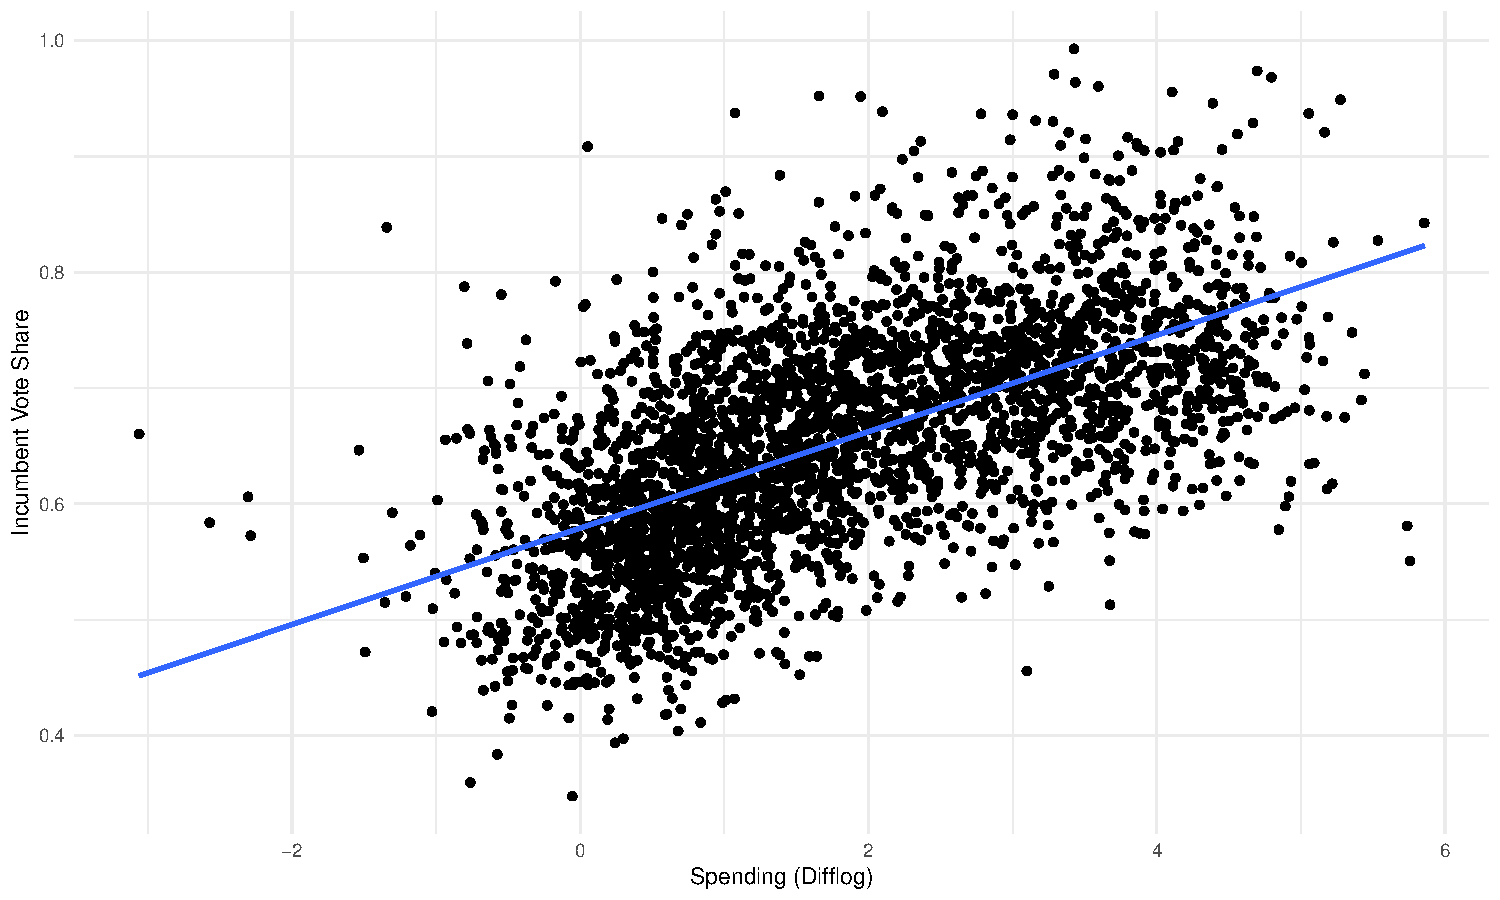
\includegraphics[width=.85\textwidth]{plot_1.pdf}
			\end{figure}
		\item Save the residuals of the model in a separate object.	\vspace{.1cm}
			\lstinputlisting[language=R, firstline=67, lastline=67]{PS03_SVU.R}  
		\item Write the prediction equation.\vspace{.5cm}
			\begin{center}
				\(Y_{1} = \alpha_{1} + \beta_{1}X = 0.579 + 0.042X\) \\
			\end{center}
			\vspace{.25cm}
		
				In R:\\
					\lstinputlisting[language=R, firstline=73, lastline=81]{PS03_SVU.R}  

	\end{enumerate}
	
\newpage

\section*{Question 2}
\noindent We are interested in knowing how the difference between incumbent and challenger's spending and the vote share of the presidential candidate of the incumbent's party are related.\\
	\begin{enumerate}
		\item Run a regression where the outcome variable is \texttt{presvote} and the explanatory variable is \texttt{difflog}. \vspace{.1cm}
			\lstinputlisting[language=R, firstline=93, lastline=93]{PS03_SVU.R}  
		\vspace{.15cm}
				\begin{table}[!htbp] \centering 
					\caption{Presidental Vote Share Explained by Spending} 
					\label{} 
					\begin{tabular}{@{\extracolsep{5pt}}lc} 
						\\[-1.8ex]\hline 
						\hline \\[-1.8ex] 
						& \multicolumn{1}{c}{\textit{Dependent variable:}} \\ 
						\cline{2-2} 
						\\[-1.8ex] & Presvote \\ 
						& Coefficients (Reg 2) \\ 
						\hline \\[-1.8ex] 
						Spending (Difflog) & 0.024$^{***}$ \\ 
						& (0.001) \\ 
						& \\ 
						Constant & 0.508$^{***}$ \\ 
						& (0.003) \\ 
						& \\ 
						\hline \\[-1.8ex] 
						Observations & 3,193 \\ 
						R$^{2}$ & 0.088 \\ 
						Adjusted R$^{2}$ & 0.088 \\ 
						Residual Std. Error & 0.110 (df = 3191) \\ 
						F Statistic & 307.715$^{***}$ (df = 1; 3191) \\ 
						\hline 
						\hline \\[-1.8ex] 
						\textit{Note:}  & \multicolumn{1}{r}{$^{*}$p$<$0.1; $^{**}$p$<$0.05; $^{***}$p$<$0.01} \\ 
					\end{tabular} 
				\end{table} 
		\item Make a scatterplot of the two variables and add the regression line. 	\vspace{.1cm}
				\begin{figure}[h!]\centering
					\caption{\footnotesize Presvote vs Difflog.}
					\label{fig:plot_2}
					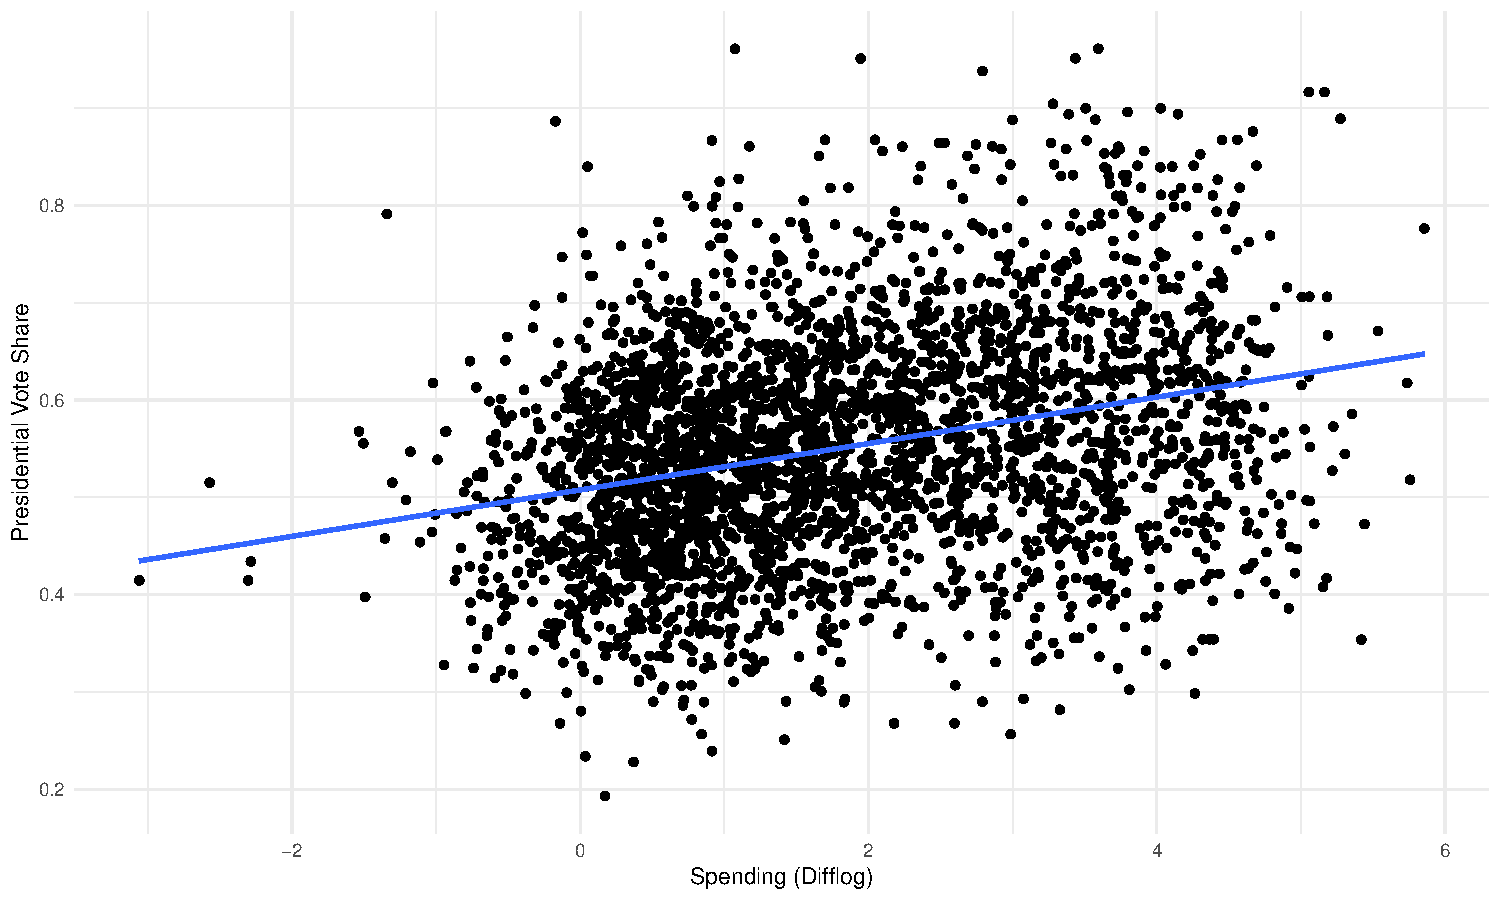
\includegraphics[width=.85\textwidth]{plot_2.pdf}
				\end{figure}
				\newpage
		\item Save the residuals of the model in a separate object.	\vspace{.25cm}
			\lstinputlisting[language=R, firstline=115, lastline=115]{PS03_SVU.R}  
		\item Write the prediction equation.\\
			\begin{center}
				\(Y_{2} = \alpha_{2} + \beta_{2}X = 0.508 + 0.024X\) \\
		\vspace{.25cm}
			\end{center}
				In R:\\
					\lstinputlisting[language=R, firstline=119, lastline=127]{PS03_SVU.R}  
		
	\end{enumerate}
	
	\newpage	
\section*{Question 3}

\noindent We are interested in knowing how the vote share of the presidential candidate of the incumbent's party is associated with the incumbent's electoral success.
	\vspace{.25cm}
	\begin{enumerate}
		\item Run a regression where the outcome variable is \texttt{voteshare} and the explanatory variable is \texttt{presvote}.
			\vspace{.1cm}
			\lstinputlisting[language=R, firstline=139, lastline=139]{PS03_SVU.R}  
			\vspace{.15cm}
		\begin{table}[!htbp] \centering 
			\caption{Incumbent Vote Share Explained by Presidential Vote Share} 
			\label{} 
			\begin{tabular}{@{\extracolsep{5pt}}lc} 
				\\[-1.8ex]\hline 
				\hline \\[-1.8ex] 
				& \multicolumn{1}{c}{\textit{Dependent variable:}} \\ 
				\cline{2-2} 
				\\[-1.8ex] & Voteshare \\ 
				& Coefficients (Reg 3) \\ 
				\hline \\[-1.8ex] 
				Presvote & 0.388$^{***}$ \\ 
				& (0.013) \\ 
				& \\ 
				Constant & 0.441$^{***}$ \\ 
				& (0.008) \\ 
				& \\ 
				\hline \\[-1.8ex] 
				Observations & 3,193 \\ 
				R$^{2}$ & 0.206 \\ 
				Adjusted R$^{2}$ & 0.206 \\ 
				Residual Std. Error & 0.088 (df = 3191) \\ 
				F Statistic & 826.950$^{***}$ (df = 1; 3191) \\ 
				\hline 
				\hline \\[-1.8ex] 
				\textit{Note:}  & \multicolumn{1}{r}{$^{*}$p$<$0.1; $^{**}$p$<$0.05; $^{***}$p$<$0.01} \\ 
			\end{tabular} 
		\end{table} 
		\item Make a scatterplot of the two variables and add the regression line. 
			\vspace{7cm}
				\begin{figure}[h!]\centering
				\caption{\footnotesize Voteshare vs Presvote.}
				\label{fig:plot_3}
				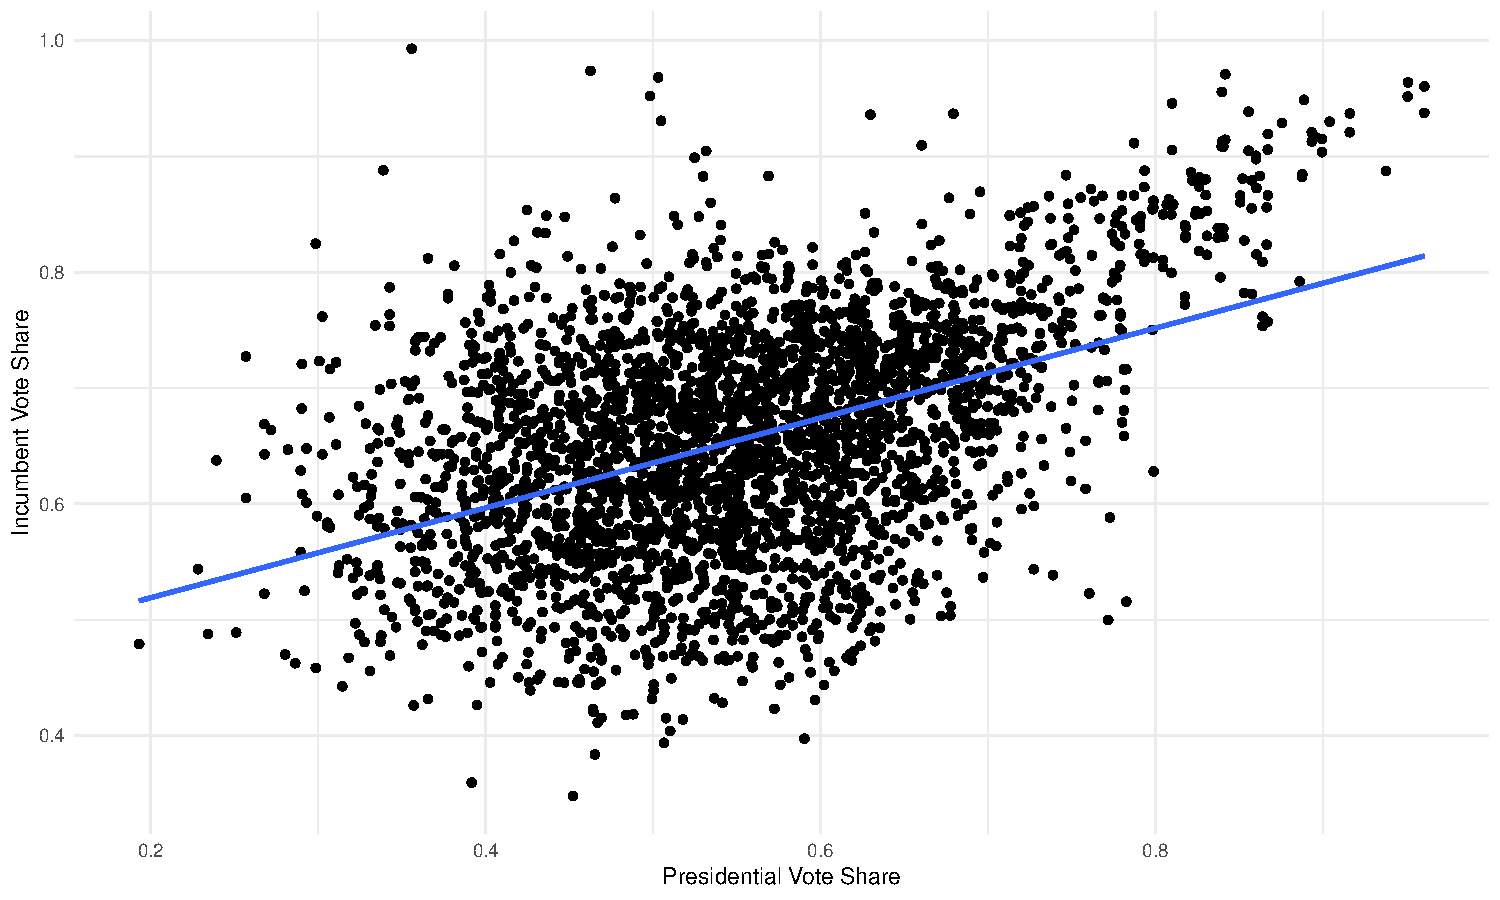
\includegraphics[width=.85\textwidth]{plot_3.pdf}
				\end{figure}
		\item Write the prediction equation.
			\begin{center}
		\(Y_{3} = \alpha_{3} + \beta_{3}X = 0.441 + 0.388X\) \\
			\end{center}
		\vspace{.25cm}
		
		In R:\\
		\lstinputlisting[language=R, firstline=161, lastline=169]{PS03_SVU.R}  
		
	\end{enumerate}
	

\newpage	
\section*{Question 4}
\noindent The residuals from part (a) tell us how much of the variation in \texttt{voteshare} is $not$ explained by the difference in spending between incumbent and challenger. The residuals in part (b) tell us how much of the variation in \texttt{presvote} is $not$ explained by the difference in spending between incumbent and challenger in the district.
	\begin{enumerate}
		\item Run a regression where the outcome variable is the residuals from Question 1 and the explanatory variable is the residuals from Question 2.	\vspace{.1cm}
		\lstinputlisting[language=R, firstline=180, lastline=180]{PS03_SVU.R}  
		\vspace{.15cm}
	\begin{table}[!htbp] \centering 
		\caption{Residuals of Reg 1 Explained by Residuals of Reg 2} 
		\label{} 
		\begin{tabular}{@{\extracolsep{5pt}}lc} 
			\\[-1.8ex]\hline 
			\hline \\[-1.8ex] 
			& \multicolumn{1}{c}{\textit{Dependent variable:}} \\ 
			\cline{2-2} 
			\\[-1.8ex] & Residuals Reg 1 \\ 
			& Coefficients (Reg 4) \\ 
			\hline \\[-1.8ex] 
			Residuals Reg 2 & 0.257$^{***}$ \\ 
			& (0.012) \\ 
			& \\ 
			Constant & $-$0.000 \\ 
			& (0.001) \\ 
			& \\ 
			\hline \\[-1.8ex] 
			Observations & 3,193 \\ 
			R$^{2}$ & 0.130 \\ 
			Adjusted R$^{2}$ & 0.130 \\ 
			Residual Std. Error & 0.073 (df = 3191) \\ 
			F Statistic & 476.975$^{***}$ (df = 1; 3191) \\ 
			\hline 
			\hline \\[-1.8ex] 
			\textit{Note:}  & \multicolumn{1}{r}{$^{*}$p$<$0.1; $^{**}$p$<$0.05; $^{***}$p$<$0.01} \\ 
		\end{tabular} 
	\end{table}
		\item Make a scatterplot of the two residuals and add the regression line. 	\vspace{6cm}
			\begin{figure}[h!]\centering
			\caption{\footnotesize Residuals 1 vs Residuals 2.}
			\label{fig:plot_4}
			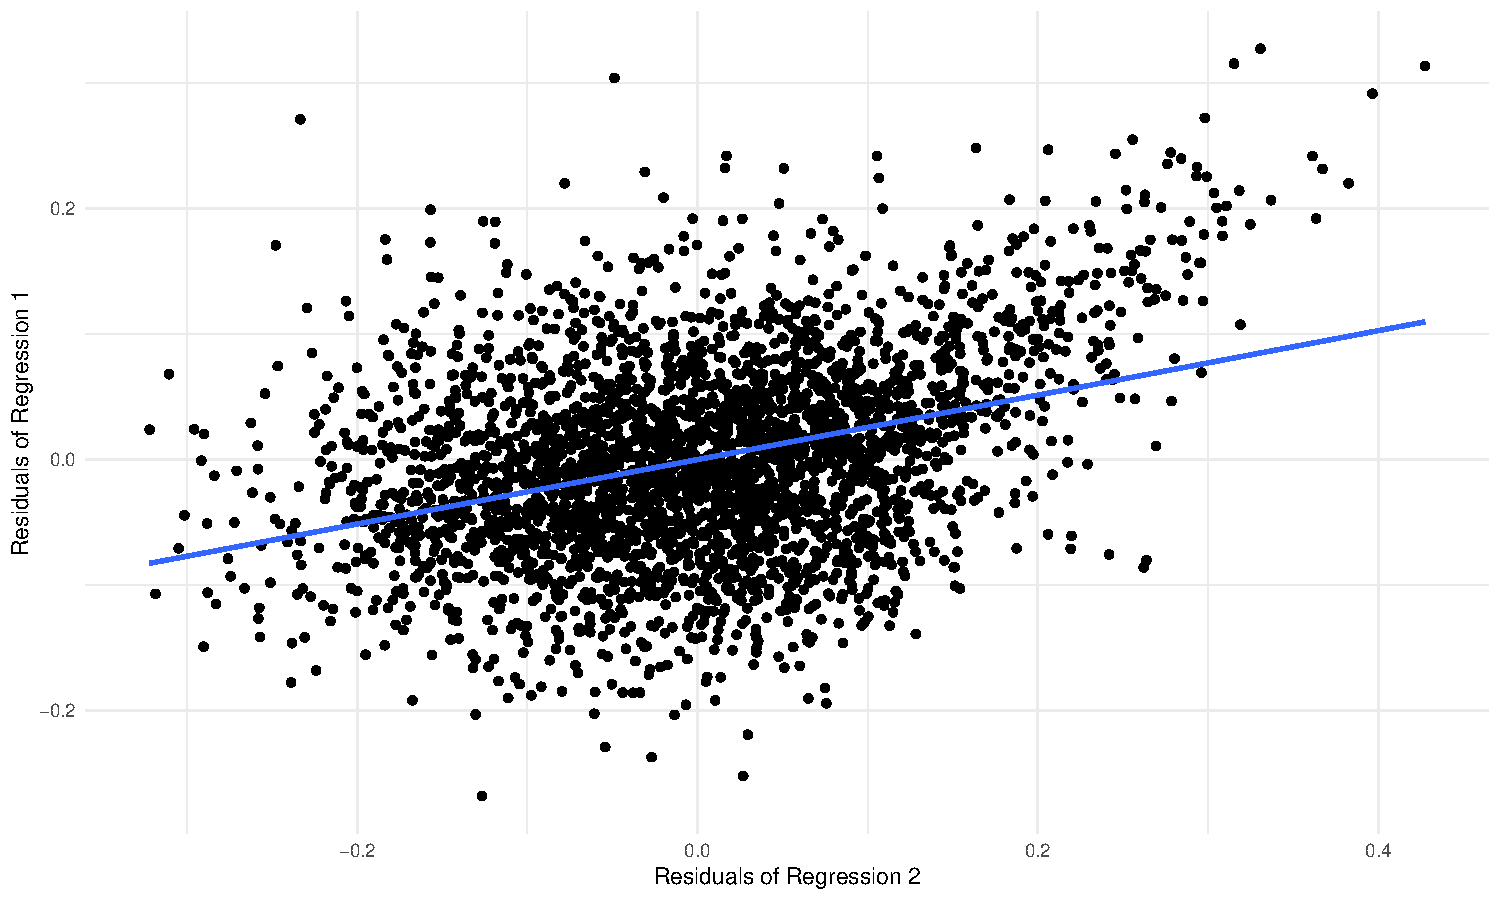
\includegraphics[width=.85\textwidth]{plot_4.pdf}
			\end{figure}
		\item Write the prediction equation.
			\begin{center}
				\(Y_{4} = \alpha_{4} + \beta_{4}X = -1.942\times10^{-18} + 0.388X\) \\
			\end{center}
		\vspace{.25cm}
		
		In R:\\
		\lstinputlisting[language=R, firstline=206, lastline=214]{PS03_SVU.R}  
		
	\end{enumerate}
	
	\newpage	

\section*{Question 5}
\noindent What if the incumbent's vote share is affected by both the president's popularity and the difference in spending between incumbent and challenger? 
	\begin{enumerate}
		\item Run a regression where the outcome variable is the incumbent's \texttt{voteshare} and the explanatory variables are \texttt{difflog} and \texttt{presvote}.	\vspace{.1cm}
		\lstinputlisting[language=R, firstline=226, lastline=226]{PS03_SVU.R}  
		\vspace{.15cm}
		\begin{table}[!htbp] \centering 
			\caption{Incumbent Vote Share Explained by Spending and Presidential Vote Share} 
			\label{} 
			\begin{tabular}{@{\extracolsep{5pt}}lc} 
				\\[-1.8ex]\hline 
				\hline \\[-1.8ex] 
				& \multicolumn{1}{c}{\textit{Dependent variable:}} \\ 
				\cline{2-2} 
				\\[-1.8ex] & Voteshare \\ 
				& Coefficients (Reg 5) \\ 
				\hline \\[-1.8ex] 
				Spending (Difflog) & 0.036$^{***}$ \\ 
				& (0.001) \\ 
				& \\ 
				Presvote & 0.257$^{***}$ \\ 
				& (0.012) \\ 
				& \\ 
				Constant & 0.449$^{***}$ \\ 
				& (0.006) \\ 
				& \\ 
				\hline \\[-1.8ex] 
				Observations & 3,193 \\ 
				R$^{2}$ & 0.450 \\ 
				Adjusted R$^{2}$ & 0.449 \\ 
				Residual Std. Error & 0.073 (df = 3190) \\ 
				F Statistic & 1,302.947$^{***}$ (df = 2; 3190) \\ 
				\hline 
				\hline \\[-1.8ex] 
				\textit{Note:}  & \multicolumn{1}{r}{$^{*}$p$<$0.1; $^{**}$p$<$0.05; $^{***}$p$<$0.01} \\ 
			\end{tabular} 
		\end{table}
		\item Write the prediction equation.	\vspace{.1cm}
			\begin{center}
				\(Y_{5} = \alpha_{5} + \beta_{difflog}X_{difflog} + \beta_{presvote}X+_{presvote} = 0.449 + 0.036X_{difflog} + 0.257X_{presvote}\) \\
			\end{center}
		\vspace{.25cm}
		
		In R:\\
		\lstinputlisting[language=R, firstline=238, lastline=246]{PS03_SVU.R}  
		
		\item What is it in this output that is identical to the output in Question 4? Why do you think this is the case?\\
		
		\vspace{.25cm}
		
			The slope (and standard error) of the Presidential Vote Share variable in the multivariate regression above is identical to the slope (and standard error) of the Residuals 2 variable (residuals of Presidential Vote Share $\sim$ Spending) when used to explain variation in the Residuals 1 variable (residuals of Incumbent Vote Share $\sim$ Spending). This makes sense, as, in steps 2 and 3, we isolate and remove the impact of Spending on Incumbent Vote Share and Presidential Vote Share to illuminate the individual impact of Presidential Vote Share on Incumbent Vote Share (holding Spending constant).\\
	\end{enumerate}




\end{document}
